\documentclass[12pt]{article}

\usepackage{graphicx}
\graphicspath{{Images/}}

\usepackage{authblk}

\usepackage{hyperref}
\hypersetup{colorlinks=true, citecolor=blue, linkcolor=blue, urlcolor=blue}

\title{\textbf{Detection of CO2 gas using NDIR gas sensor}}

\author[1, a)]{Rishav Pandey}
\affil[1]{Senior, Department of Electronics and Tele-Communication
Engineering, Jabalpur Engineering College, Jabalpur-482011,
India.}
\affil[a)]{Corresponding author: rishav160999@gmail.com}

\date{Report submitted to\\ CSIR-Central Electronics Engineering Research Institute\\ for the completion of Research Internship\\ under the guidance of\\ Dr. Vijay Chatterjee, Sr. Scientist, CSIR-CEERI}


\providecommand{\ProjectDuration}{\textbf{Project Duration: }}

\usepackage{pdfpages}

\begin{document}

\maketitle
\ProjectDuration{July 7, 2021 - December 31, 2021}
\clearpage

\tableofcontents
\clearpage
\listoffigures
\clearpage


\section{ACKNOWLEDGEMENT}
It is my proud privilege and duty to express my sincere regards to several 
people for the kind of help and guidance received from them in preparation 
of this report. It would not have been possible to prepare this report in this 
form without their valuable help, cooperation and guidance.\\
\\
Firstly, I would thank my scientific supervisor Dr. Vijay Chatterjee for
giving me this wonderful opportunity to work on a research project under his guidance. He guided me throughout the duration of this project.\\
\\
I would also like to thank my parents and my elder brother for
continuously motivating me to complete this project successfully.\\
\\
\\
\\
\\
\\
\\
\\
\\
\\
Rishav Pandey\\
B.Tech 7th Sem,\\
Electronics \& Communication Engineering,\\
Jabalpur Engineering College

\clearpage

\section{DECLARATION}
I hereby declare that the project report entitled “Detection of CO2 gas using NDIR gas sensor” submitted by me in partial fulfillment of the 
requirement for the internship certificate from CSIR-Central Electronics Engineering Research Institute is authentic work
undertaken by me.\\
\\
I also confirm that this report is only prepared for my academic requirement not for any other purpose.\\
\\
\\
\\
\\
\\
\\
\\
\\
Rishav Pandey\\
B.Tech 7th Sem,\\
Electronics \& Communication Engineering,\\
Jabalpur Engineering College

\clearpage

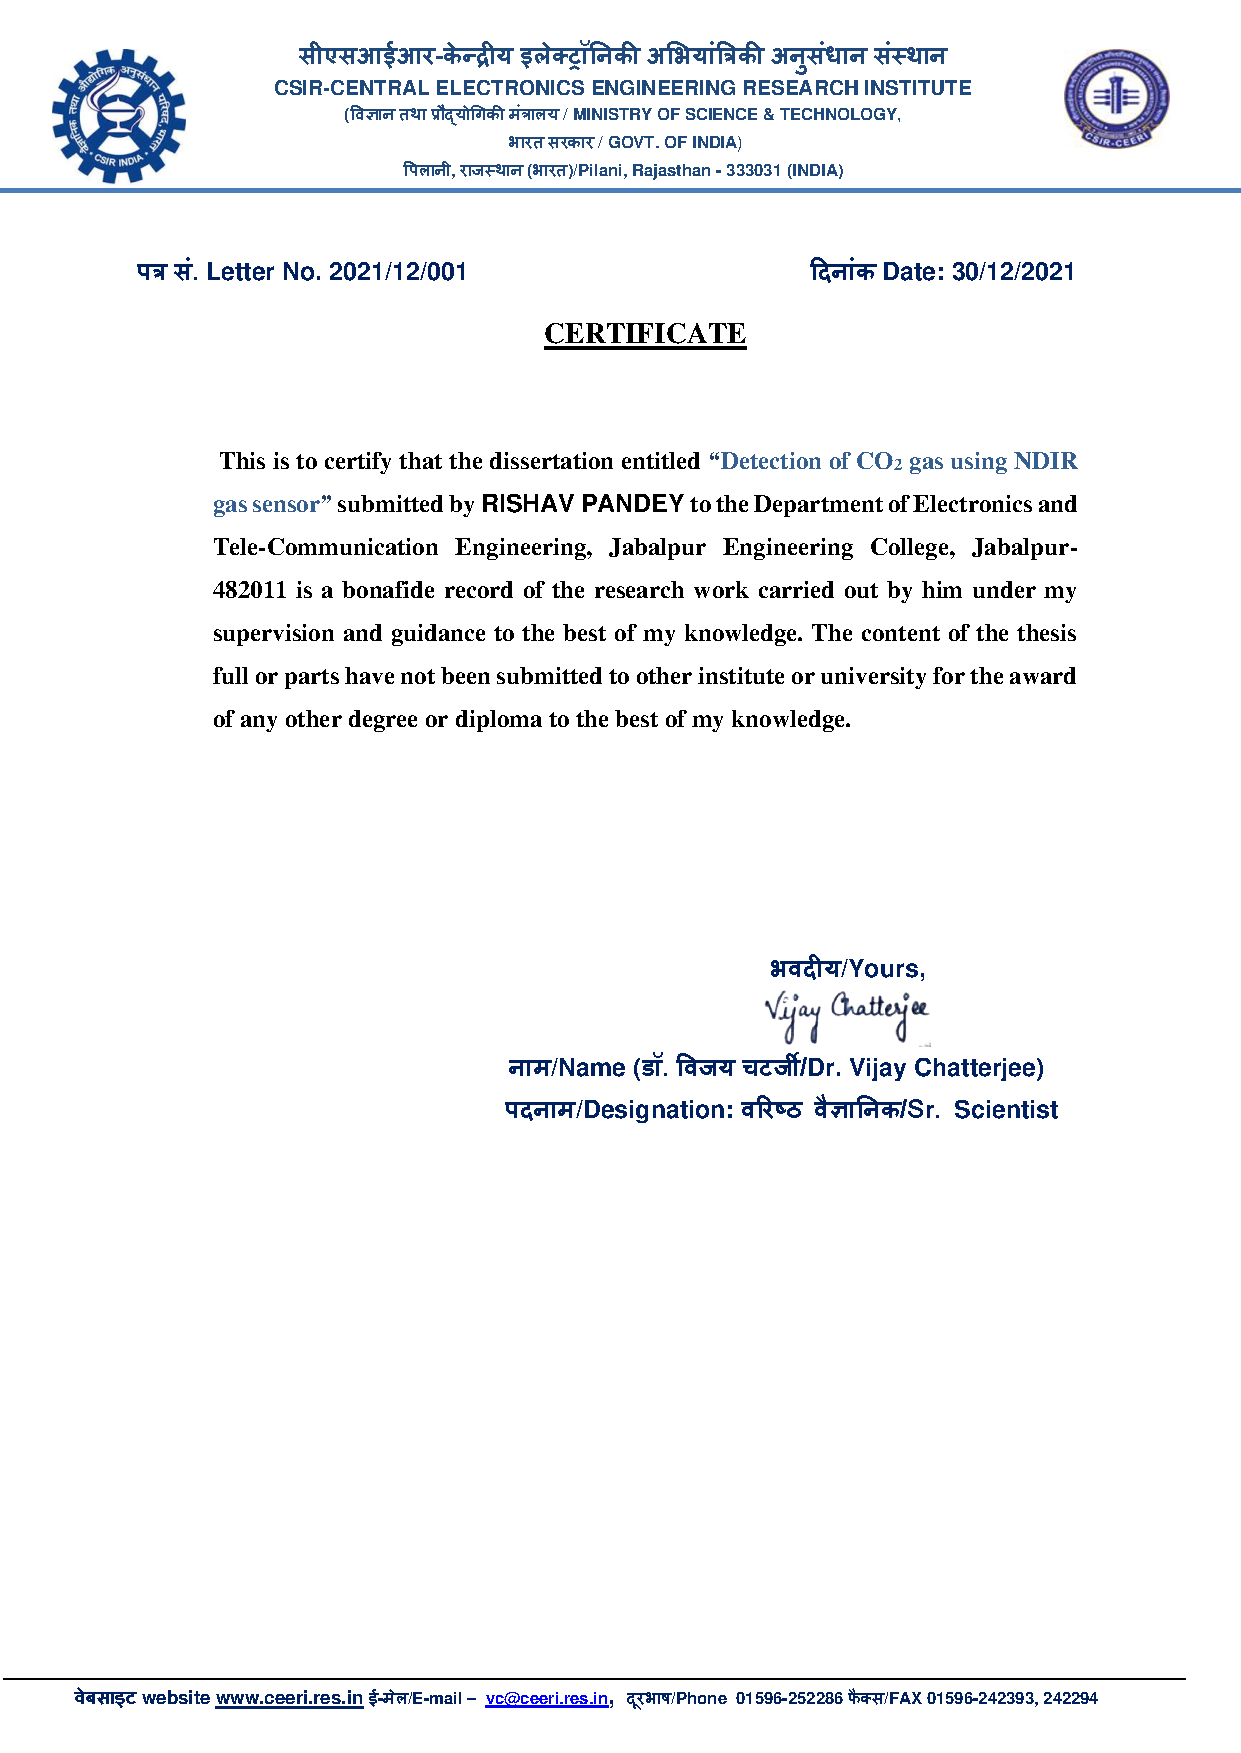
\includepdf[pages=1]{CSIR_CEERI_Certificate.pdf}

\begin{abstract}
NDIR is an industry term for "non-dispersive infrared” and is the most common 
type of sensor used to measure carbon dioxide, or CO2. However, this gas 
detector is not limited only for CO2 gas but can be used to detect any IR- Active 
gas like CO, NO, SO2 but at different wavelengths of Infrared Radiation. It is 
called as Non-Dispersive because the IR light which passes through the gas 
chamber is not pre-filtered.
In NDIR Gas Sensors, generally two main things happen:\\
1. Beer-Lambert Law\\
2. IR-Spectroscopy\\
Since, the Infrared Radiation passes through a cylindrical gas chamber, its 
intensity varies exponentially as the length of the chamber and the 
concentration of CO2 increases. Thus, showing an application of Beer-Lambert 
Law. We can also see an interaction of IR light with the CO2 gas molecules, so we 
can say there is an involvement of IR-Spectroscopy in this project. 
NDIR gas sensor consists of an infrared source, detector, optical filter, gas cell, 
and electronics for signal processing. A single light source, dual wavelength type 
gas sensor has two detectors and two optical filters of different wavelengths 
which are placed in front of each detector. Before passing the CO2 gas we see 
the decrease in intensity of IR radiation (in the absence of IR active gas). This 
decrease in radiation is because of the length of the gas cell. Now, we pass CO2 
gas through the inlet and simultaneously we pass the IR light, in this case the 
intensity of IR light decreases further because of the interaction of CO2 gas 
molecules with the same. It may be noted that the Infrared Radiation of 
wavelength ranging from 0.7 $\mu$m to 1 mm is passed through the gas cell. 
However, the CO2 gas molecules interact at a wavelength of around 4.26 $\mu$m
causing vibration of the gas molecules.
Some, of the infrared light is absorbed by the target gas while some IR radiation 
passes without any absorption. One that is absorbed by a target gas passes 
through the active filter with a particular bandwidth for the detection of the 
target gas while the other which does not interact with the target gas passes 
through the reference filter. NDIR gas sensor detects the decrease in 
transmitted infrared light which is in proportion to gas concentration. The 
difference between transmitted light intensities in these two bandwidths is 
converted into gas concentration. In this way, we can calculate the 
concentration of CO2 gas present in a gas chamber. 
While there are multiple methods, through which a target gas can be detected 
by an NDIR gas sensor like using Photodetectors such as Photoconductivity Cell
or using Thermal Detectors such as Pyroelectric detectors, Thermopile, 
Thermistor, Bolometer and Golay Cell. However, in this project we are limited 
only to pyroelectric detector for the detection of target gas.
This project finds multiple applications in industries as well as in normal 
households. It can also be used to track the concentration of CO2 gas in a room 
present with NDIR gas sensor. As according to the World Health Organization, 
increased level of CO2 gas in environment can increase the risk of transmission 
of SARS-CoV-2 virus. In any given indoor environment, when CO2 level doubles, 
the risk of transmission also roughly doubles. The same has been confirmed by 
the researchers of Cooperative Institute for Research in Environmental Sciences 
(CIRES) and the University of Colorado Boulder. So, monitoring the level of CO2
gas in a room through this project can be an inexpensive and wonderful way to 
prevent the transmission of Covid-19 virus.
\end{abstract}
\clearpage

\section{INTRODUCTION}
A nondispersive infrared sensor (also known as an NDIR sensor) is a basic spectroscopic sensor that is frequently employed as a gas detector. It is non-dispersive because no dispersive device (such as a prism or diffraction grating) is employed to split the broadband light into a narrow spectrum suited for gas sensing (as is common in other spectrometers). A broadband light source and an optical filter are used in the majority of NDIR sensors to choose a narrow band spectral area that overlaps the absorption region of the gas of interest. In this case, a 50-300nm bandwidth may be considered narrow. Microelectromechanical systems (MEMs) or mid-IR LED sources may be used in modern NDIR sensors, which can be used with or without an optical filter.
An infrared (IR) source (lamp), a sample chamber or light tube, a light filter, and an infrared detector are the primary components of an NDIR sensor. The IR light passes through the sample chamber and is directed towards the detector. In a separate chamber, a reference gas, usually nitrogen, is enclosed. According to the Beer–Lambert equation, the gas in the sample chamber absorbs particular wavelengths, and the detector measures the attenuation of these wavelengths to estimate the gas concentration. In front of the detector is an optical filter that filters out all light except that which the chosen gas molecules can absorb.
Other gas molecules should ideally not absorb light at this wavelength and hence have no effect on the amount of light reaching the detector, although cross-sensitivity is unavoidable.  Many IR measurements are cross sensitive to H2O, for example, therefore gases like CO2, SO2, and NO2 frequently cause cross sensitivity at low concentrations.

\section{BEER LAMBERT LAW}

The operating principle of NDIR gas sensor is governed by Beer Lambert Law.

\subsection{LAMBERT LAW}
When a beam of  monochromatic light passes through an absorbing medium then its intensity decreases exponentially as the length of the absorbing medium increases.
$$I=I_{0}e^{-kl}$$ 

\subsection{LAMBERT BEER LAW}
When a beam of  monochromatic light passes through an absorbing medium then its intensity decreases exponentially as the length and concentration of the absorbing medium increases.

$$I=I_{0}e^{-kcl}$$ 

\begin{figure}[h]
\centering
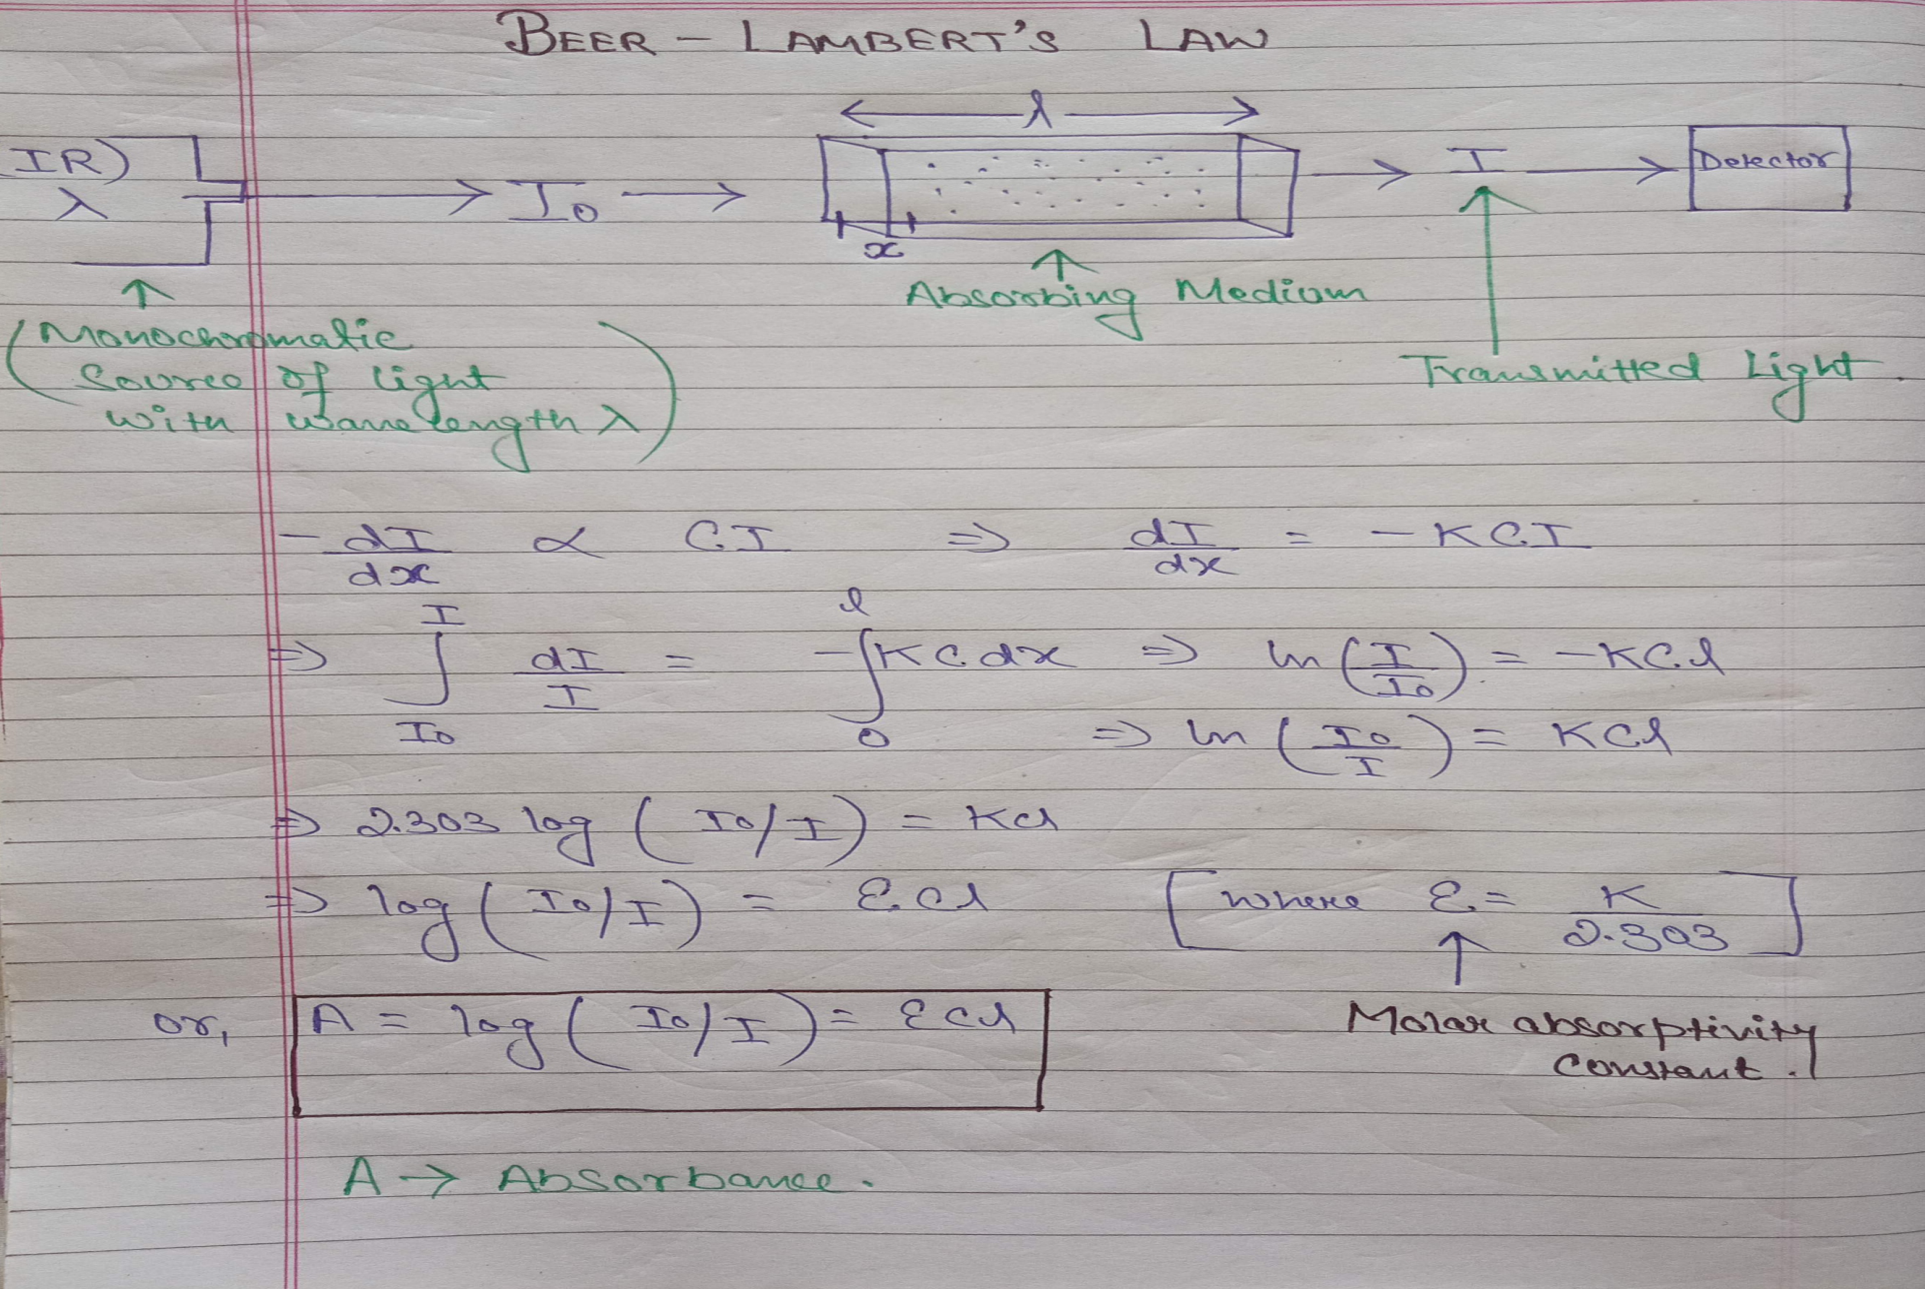
\includegraphics[scale=0.7]{Beer.png}
\caption{Derivation of Beer Lambert Law}
\end{figure}

\begin{figure}[h]
\centering
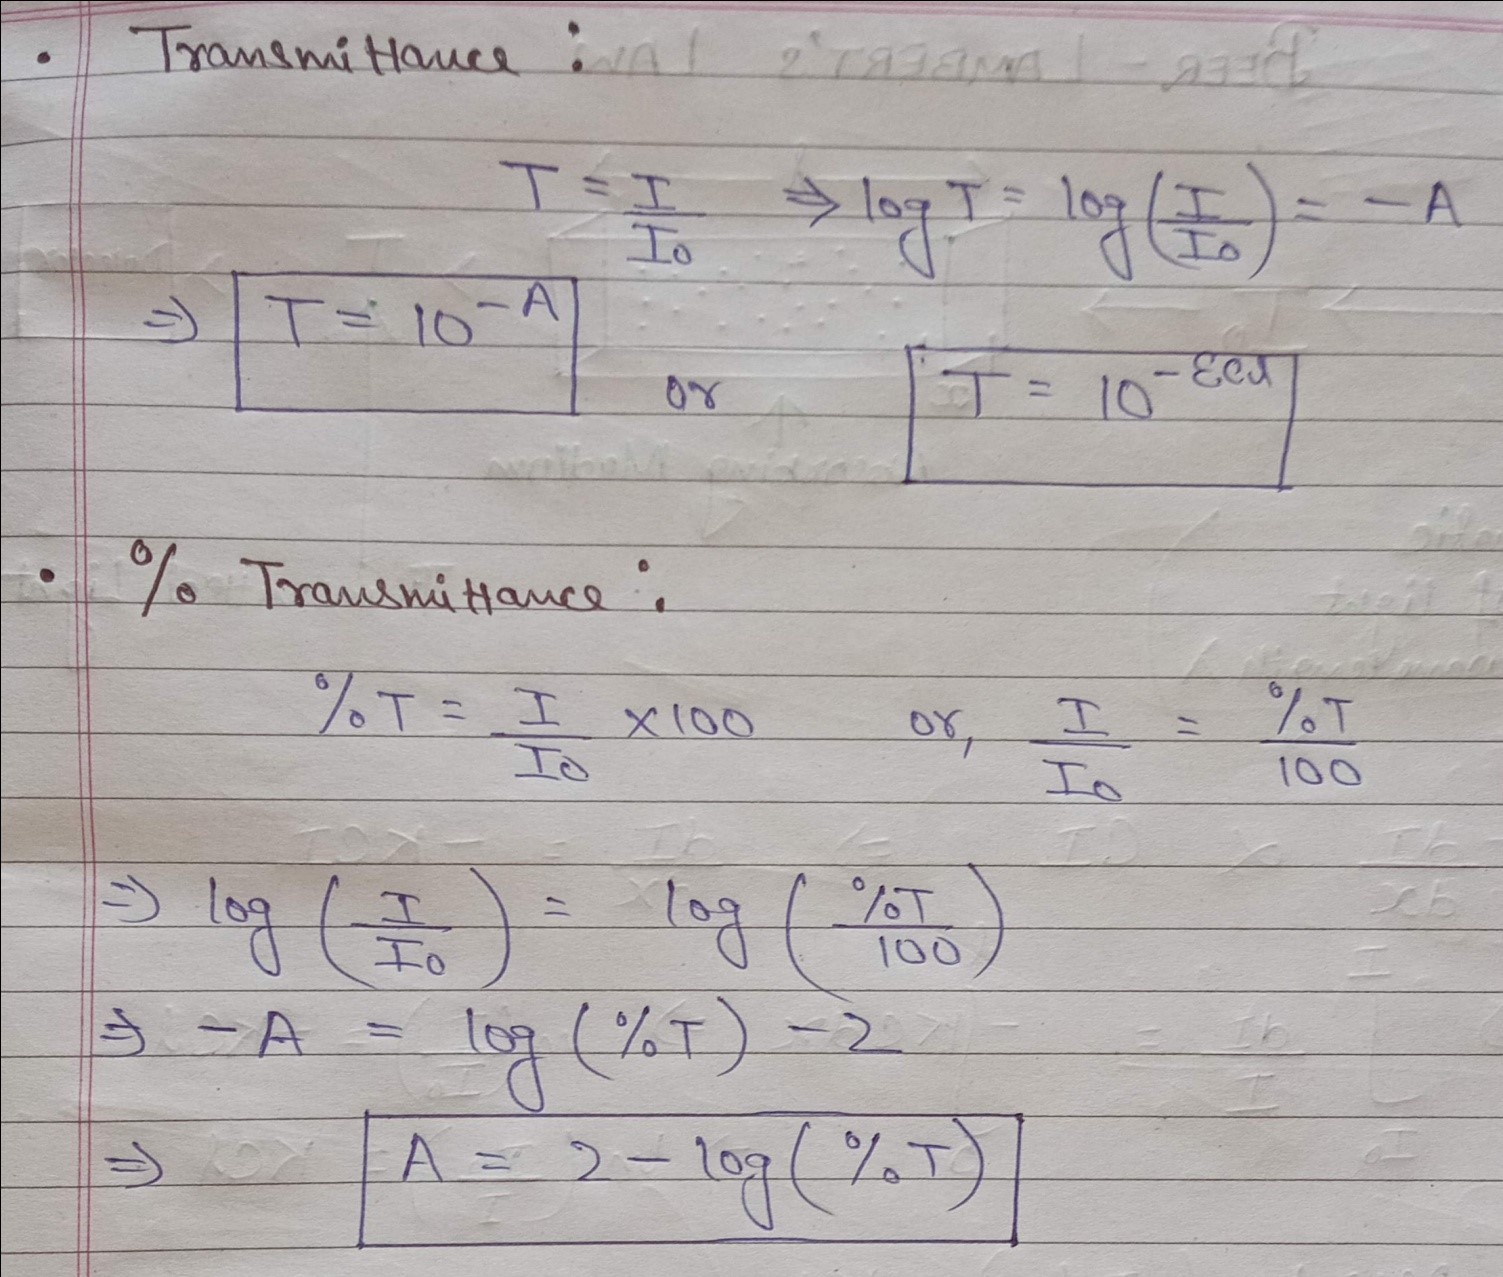
\includegraphics[scale=0.7]{lambert.jpg}
\caption{Calculation of Transmittance}
\end{figure}

\section{OPERATING PRINCIPLE}
When infrared radiation interacts with gas molecules, infrared light is absorbed by the gas molecules at a particular wavelength, causing vibration of the gas molecules. NDIR gas sensors detects the decrease in transmitted infrared light which is in proportion to gas concentration. This transmittance, the ratio of transmitted radiation energy to the incident energy, is dependent on target gas concentration.

\begin{figure}[h]
\centering
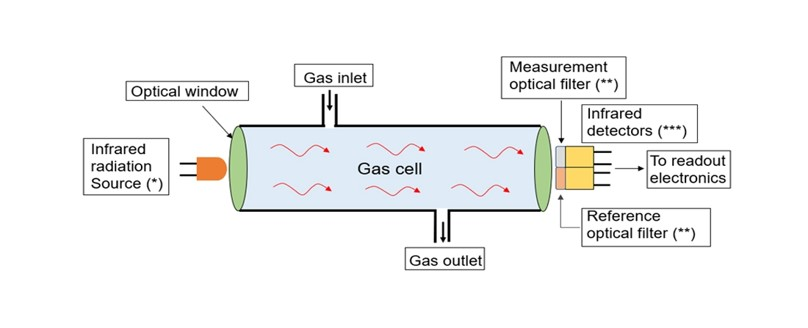
\includegraphics[scale=0.7]{NDIR.jpg}
\caption{Schematic view of NDIR gas sensor}
\end{figure}

NDIR gas sensor consist of an infrared source, detector, optical filter, gas cell, and electronics for signal processing. A single light source, dual wavelength type gas sensor has two detectors and two optical filters of different wavelengths which are placed in front of each detector. Infrared light that is absorbed by a target gas passes through the active filter with a particular bandwidth for the detection of the target gas. Infrared light that does not interact with the target gas passes through the reference filter. The difference between transmitted light intensities in these two bandwidths is converted into gas concentration.

\begin{figure}[h]
\centering
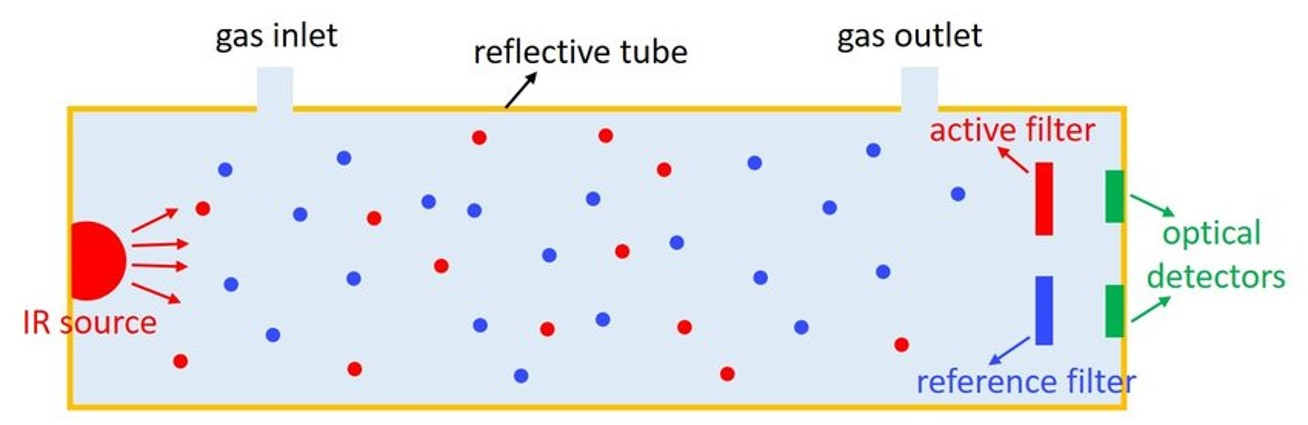
\includegraphics[scale=0.7]{NDIR1.jpg}
\caption{NDIR gas sensor using optical detectors}
\end{figure}

\section{ABSORPTION SPECTRUM}
Most of the gases absorbs the Mid infrared radiation from 2.5µm to 12µm. the gases like water vapour (H2O), Carbon di oxide (CO2), Carbon monoxide (CO), Nitrogen di Oxide (NO2), Ozone (O3) etc absorbs the infrared radiation at a particular wavelength. From these absorption spectrum carbon di Oxide (CO2) absorbs the 4.2µm of wavelength in the Infrared radiation. In this project we use this wavelength to detect the Carbon di Oxide gas present in the chamber. From fig. \ref{Absorption spectrum of different IR active gases}, we observe that the absorption of IR radiation by CO2 gas molecules becomes maximum at 4.26 $\mu$m 

\begin{figure}[h]
\centering
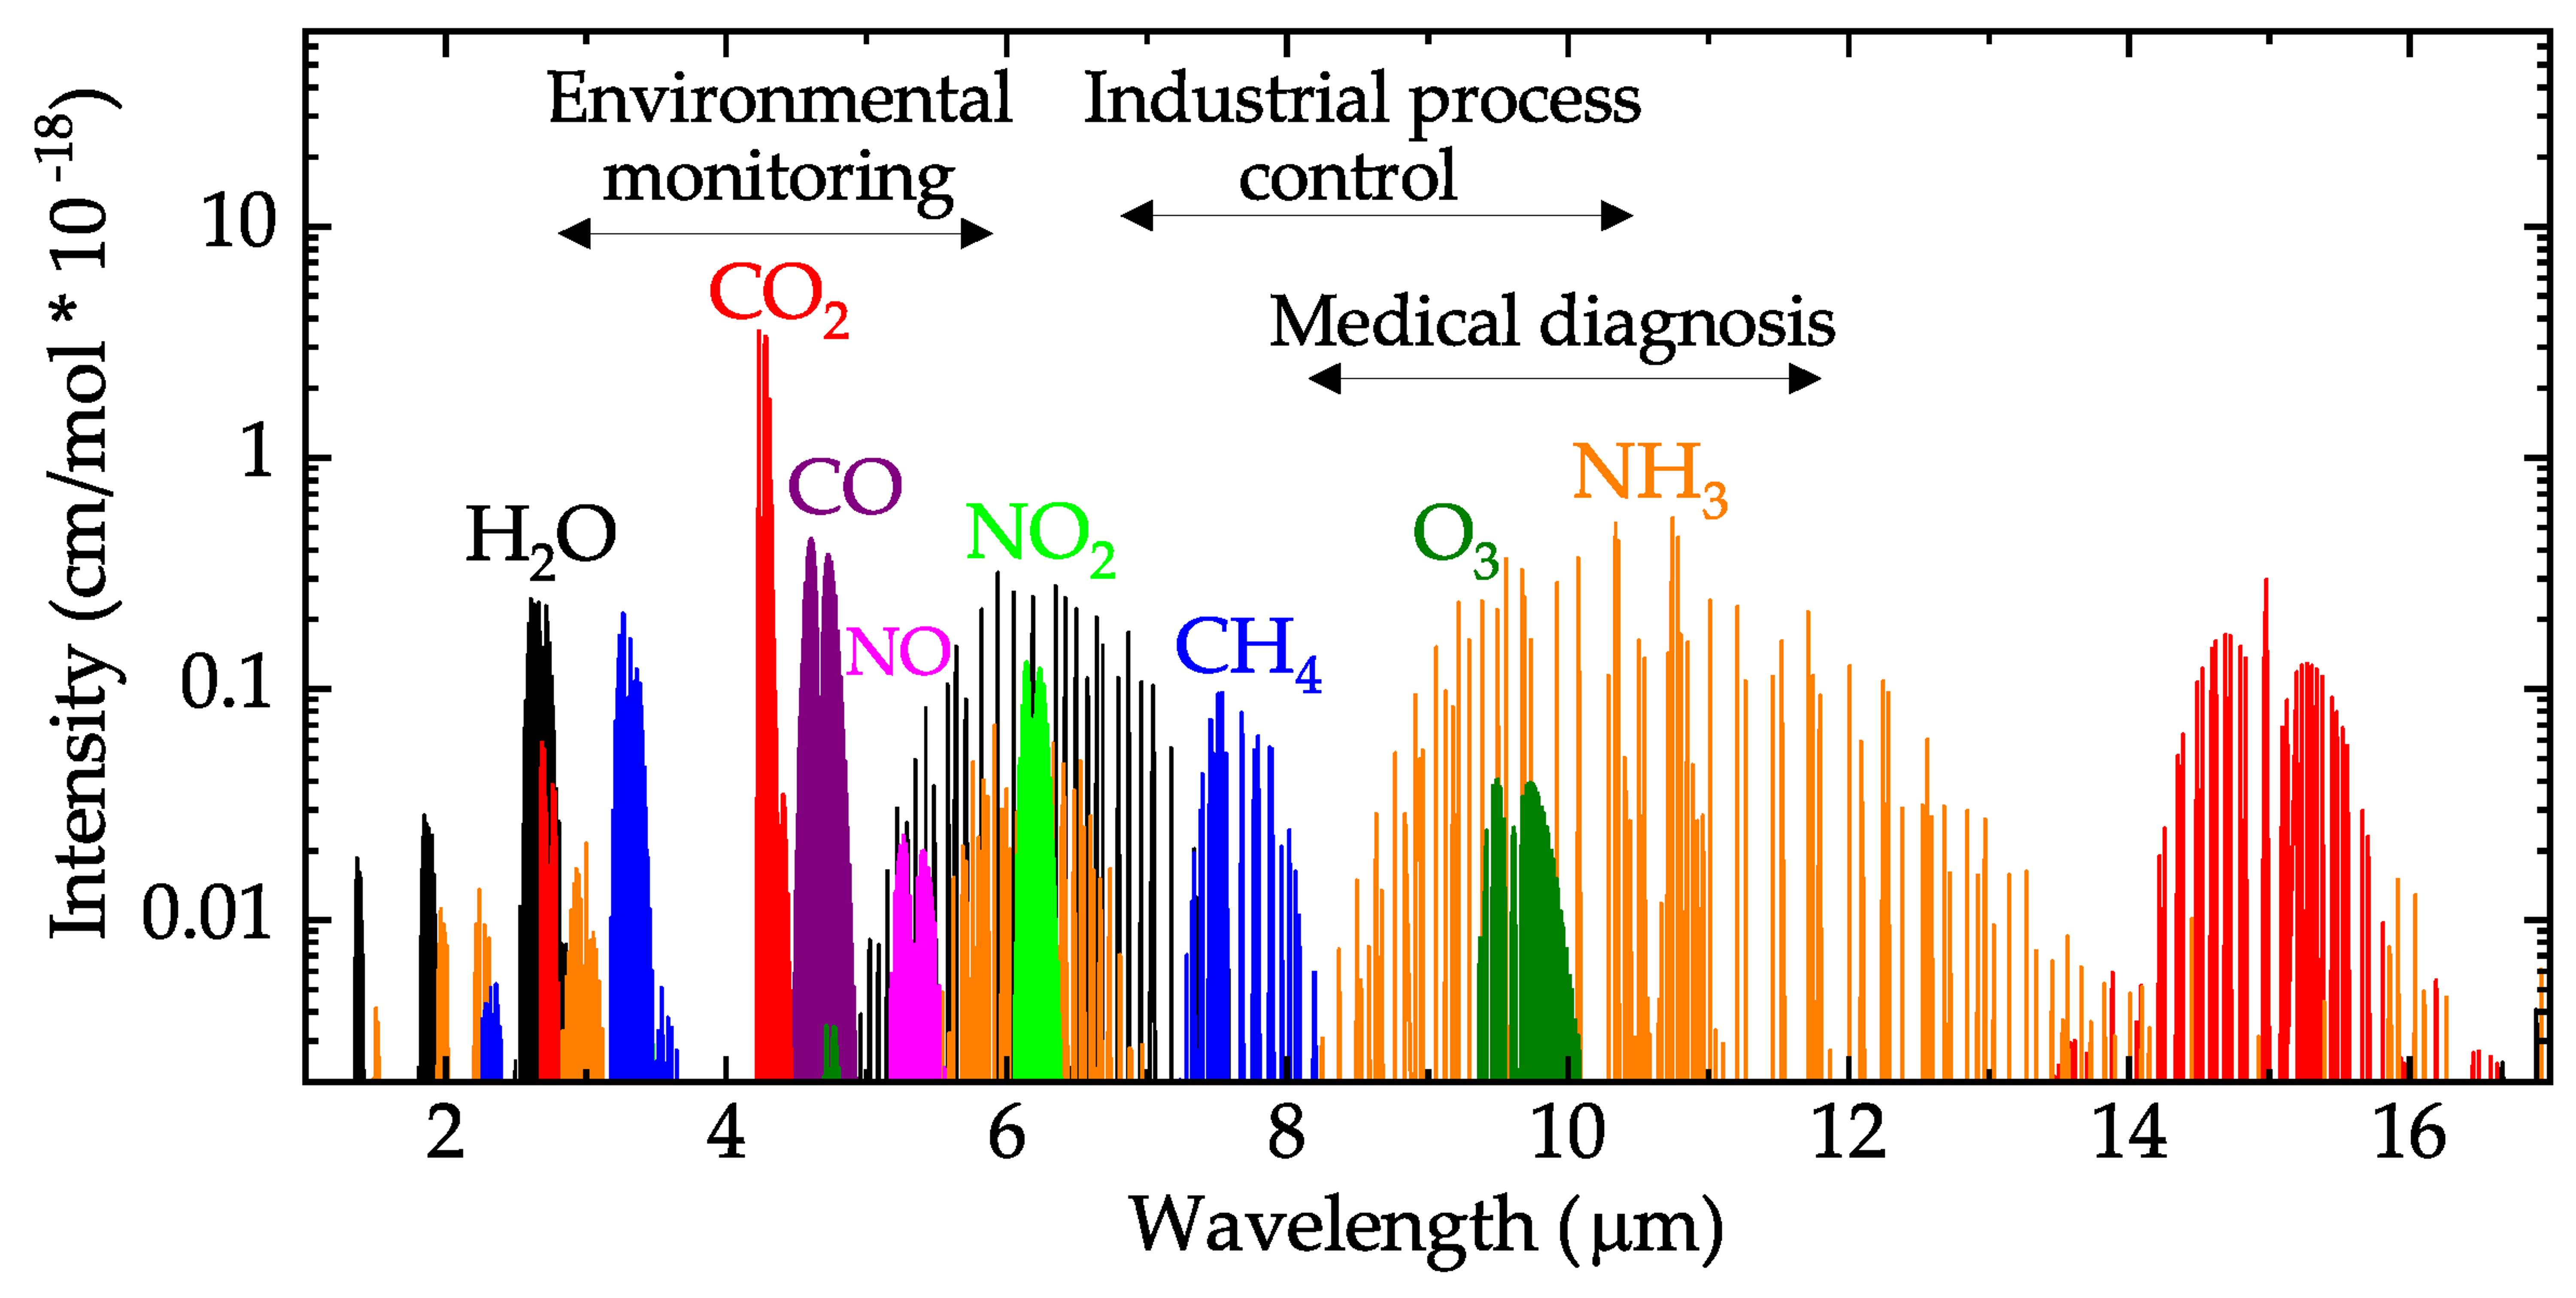
\includegraphics[scale=0.55]{absorption spectrum.png}
\caption{Absorption spectrum of different IR active gases}
\label{Absorption spectrum of different IR active gases}
\end{figure}

\section{METHODOLOGY}
We use the NDIR approach, based on optical gas sensing, leveraging 
the change in light intensity when CO2 gas molecules interact with light. 
As CO2 gas molecules have a characteristic absorption line in the mid-infrared (IR) spectral region, a drop in the transmitted signal due 
to CO2 gas molecules absorption is expected when light passes through 
the CO2 gas. This drop in signal will eventually be read as an electrical 
signal related to the gas sensitivity and CO2 gas concentration. The 
wavelength of 4.26 $\mu$m is chosen for CO2 gas absorption in this work as 
CO2 gas presents strong absorption peaks at wavelength of 4.26 $\mu$m\cite{ng2021ndir}. This 
is also the mid-IR wavelength with minimal or negligible overlap of CO2 
absorption peaks with other gases commonly present in ambient air. NDIR approach will work for gases like CO2 which are IR active, 
where a change in its dipole moment result in an oscillating electric 
field. The electric vector of the electromagnetic radiation which oscillates at the same frequency as the oscillating electric field due to change 
in dipole moment will be absorbed by the gas molecule. Atomic species 
such as argon (Ar) and homonuclear diatomics such as oxygen (O2) and 
N2 are not IR active and will not absorb IR radiation. Ar has only one 
atom and thus cannot exhibit a dipole moment. O2 and N2 have adjacent 
atoms with identical electro-negativities – vibration and rotation do not 
result in a change in their dipole moment. 
NDIR sensing requires a source emitting wavelengths at the absorption line of the targeted gas, and a detector for sensing the signal change. 
For the source, we chose a blackbody radiation source which emits a wide 
spectrum of wavelengths and hence can cover the absorption lines of 
many gases. By choosing appropriate optical filters, this blackbody radiation source could be used as the emitting source for detection of 
different specific gases. Using a blackbody radiation source with an 
appropriate optical filter is relatively low cost compared to using QCL and 
LED sources which emit only at particular wavelengths. In this paper, as 
we are detecting CO2 gas using CO2 absorption wavelength at 4.26 $\mu$m, 
an optical bandpass filter centered at wavelength of 4.26 $\mu$m is used. For 
the detector, we use our in-house fabricated ScAlN-based pyroelectric 
detector operating at room temperature and atmospheric pressure, and is 
able to detect over a wide range of spectral wavelengths. 


\begin{figure}[h]
\centering
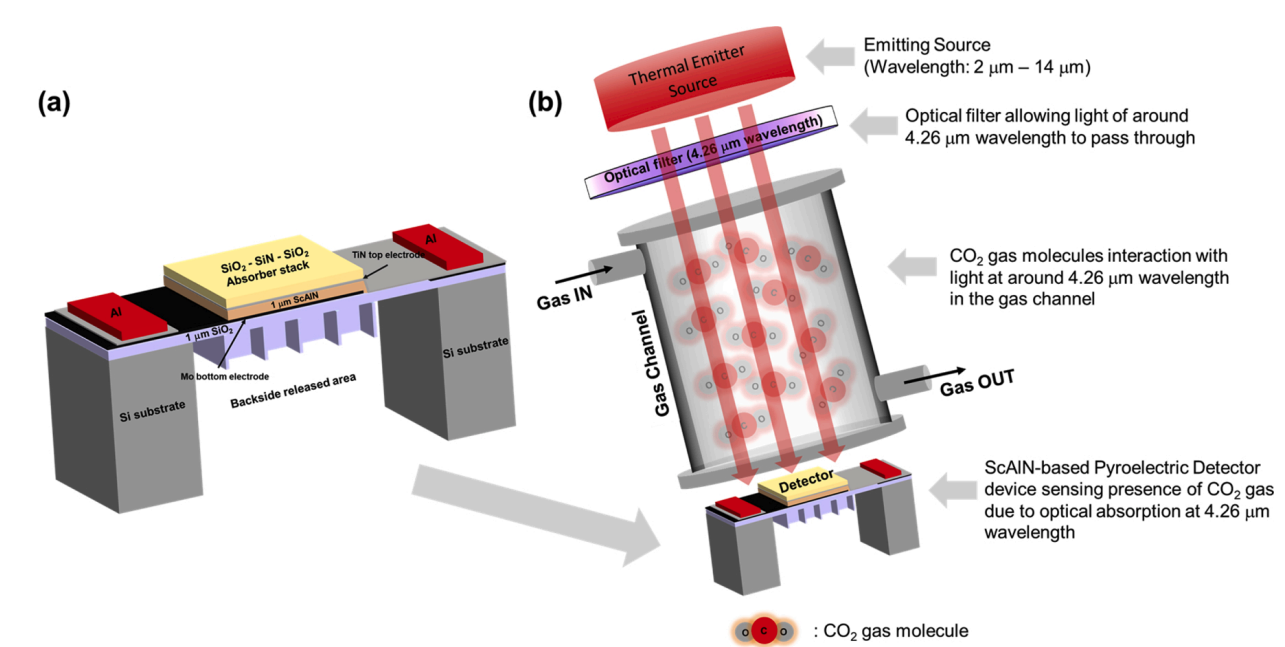
\includegraphics[scale=0.5]{NDIR gas sensor with pyro.png}
\caption{NDIR gas sensor using pyroelectric detector}
\label{NDIR gas sensor using pyroelectric detector}
\end{figure}

Fig. \ref{NDIR gas sensor using pyroelectric detector} shows a schematic of the ScAlN-based pyroelectric detector 
that we use. The pyroelectric detector consists of a pyroelectric sensing 
layer with area 500 $\mu$m x 500 $\mu$m. We use 12 \% doped ScAlN with 
thickness of 1 $\mu$m as the pyroelectric sensing layer\cite{ranacher2019cmos}. On top and below the 
ScAlN sensing layer is the top and bottom electrodes respectively. Titanium nitride (TiN) is used as the top electrode and molybdenum (Mo) as 
the bottom electrode. Above TiN top electrode is a dielectric stack of 
silicon dioxide – silicon nitride – silicon dioxide (SiO2-SiN-SiO2) which 
acts as the absorber to help enhance light absorption into the device. This 
absorber stack is used to help broaden the absorption bandwidth with 3 
layers of dielectric films and create destructive light wave interference in the stack for more efficient absorption. The top and bottom electrodes are connected to aluminum metal pads which act as metal contacts 
for electrical connections. Below the bottom electrode is a 1 $\mu$m thick 
SiO2 layer with waffle-like structures\cite{hyseni2010analysis}. The SiO2 material helps to thermally isolate the thermal energy received by the pyroelectric detector 
sensing layer, slowing down thermal conduction to the medium below. In 
addition, the Si substrate is released from the backside to form an air 
cavity area under the pyroelectric sensing region to further reduce thermal losses as air is a poor thermal conductor. The SiO2 waffle-like 
structures (also called SiO2 ribs) help to increase the mechanical stiffness of the pyroelectric sensing region which is in membrane form\cite{odon2010modelling}. 
The fabrication steps of ScAlN-based pyroelectric detectors and their 
electrical characteristics are reported elsewhere in literature. 

\section{RESULTS}
At different concentration of CO2 gas enclosed in a gas cell, we have obtained the percentage decrease in the intensity of IR radiation which is due to the absorption of IR radiation by CO2 gas molecules. 

\begin{figure}[h]
\centering
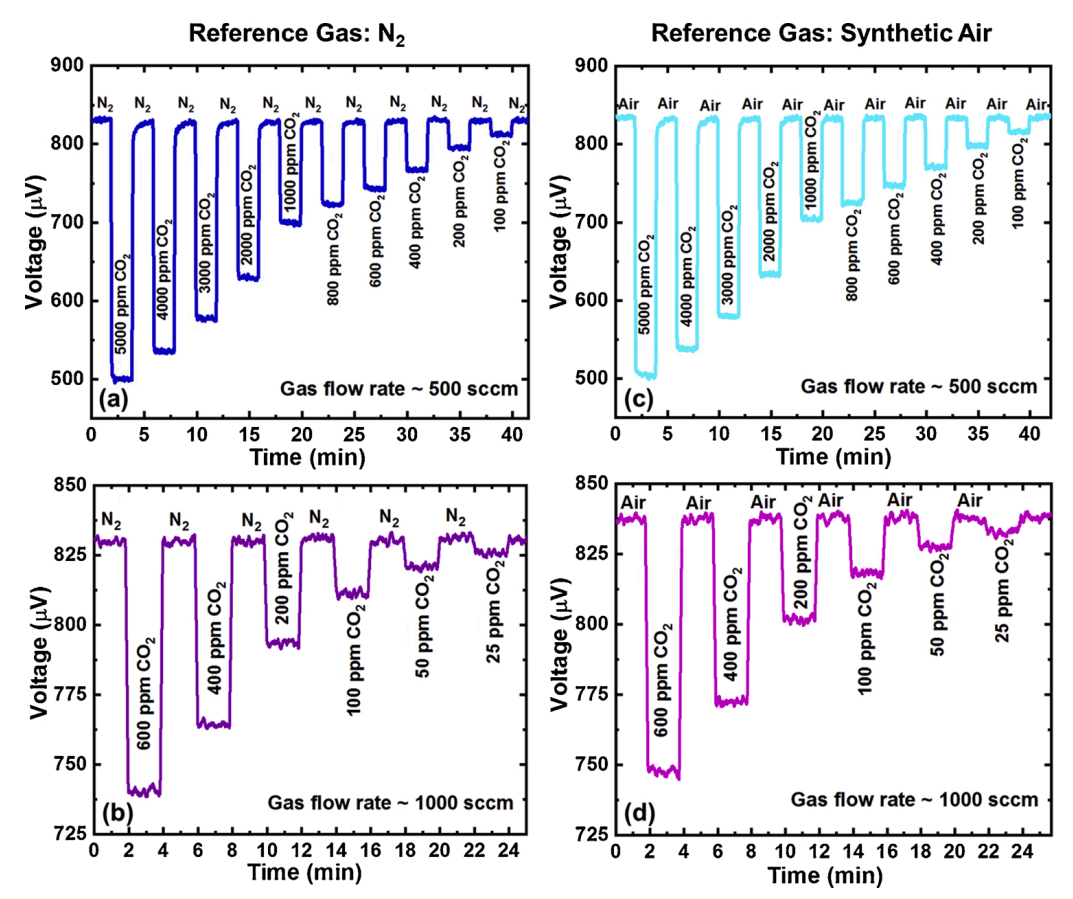
\includegraphics[scale=0.5]{gas response.png}
\caption{CO2 gas response at different conc. of CO2 gas}
\label{CO2 gas response at different conc. of CO2 gas}
\end{figure}

\begin{figure}[h]
\centering
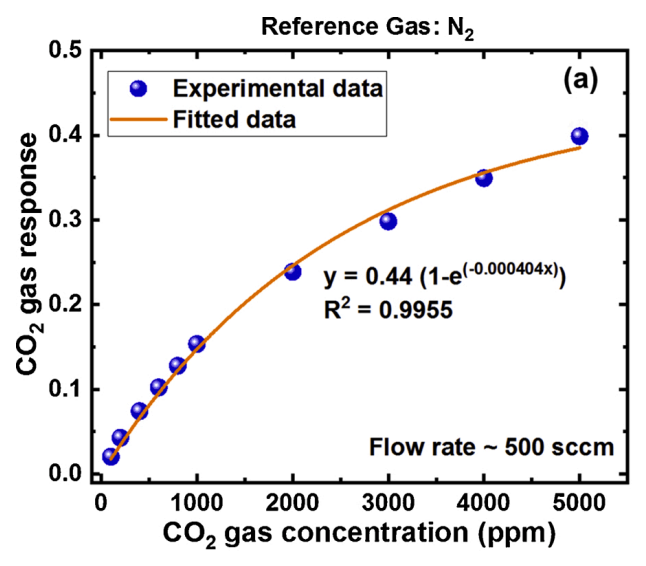
\includegraphics[scale=0.5]{CO2 gas response in presence of N2.png}
\caption{CO2 gas response with N2}
\label{CO2 gas response with N2}
\end{figure}
\clearpage


\begin{figure}[h]
\centering
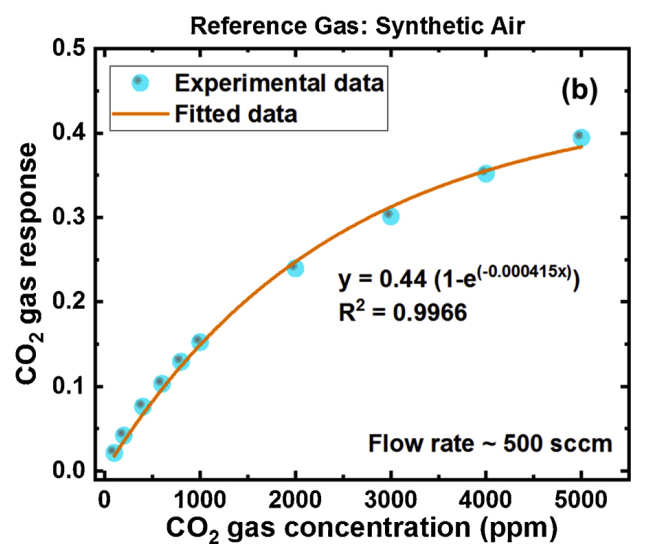
\includegraphics[scale=0.5]{CO2 gas resp in presence of SA.png}
\caption{CO2 gas response with synthetic air}
\label{NCO2 gas response with synthetic air}
\end{figure}



\section{CONCLUSION}
We have demonstrated NDIR gas sensing for CO2 gas using a CMOS 
compatible MEMS ScAlN-based pyroelectric detector. Using a blackbody 
thermal emitter source, an optical bandpass filter, a gas channel of 
length 10 cm and our in-house fabricated CMOS compatible MEMS 
ScAlN-based pyroelectric detector using 8-inch wafer technology with 
ScAlN deposition temperature at $200^{O}C$, we are able to sense changes 
in CO2 gas concentration from 5000 ppm, down to 25 ppm CO2 gas 
concentration. The different concentrations of CO2 gas are determined 
from the percentage change in the voltage signal when switching from 
the reference N2 gas or synthetic air to CO2 gas. CO2 gas responses 
measure 2\% for sensing 100 ppm CO2 concentration and 40 \% for 
sensing 5000 ppm CO2 gas concentration. The CO2 response times are 
measured when detecting 5000 ppm, 1000 ppm and 400 ppm CO2 gas 
concentrations in N2 and synthetic air respectively and the results show 
in general ~2 s or lower. Humidity introduced to the CO2 gas up to 70 \% 
relative humidity shows some minor effect (<3\%) to the CO2 gas 
response. Specifically, CO2 gas response seems to be most perturbed at 
10 \% relative humidity. The effect of humidity on CO2 gas response also 
seems to effect more on CO2 gas in N2 compared to CO2 gas in synthetic 
air\cite{tan2020non}. These measured results could serve as guidelines for practical applications in NDIR CO2 gas sensing, and are promising for CMOS 
compatible MEMS ScAlN-based pyroelectric detectors used in NDIR gas 
sensing, opening further possibilities for low cost, wafer-level monolithic NDIR gas sensors with small footprints integrable with CMOS 
circuits.
\clearpage

\bibliographystyle{elsarticle-num}
\bibliography{refer.bib}










\end{document}